%{(lambda (k)}

トンネルが間もなく近づくと、
私は習慣として、カバンから煮干しチップの小袋を一つ取り出し、
一口だけつまんで食べた.
ここのトンネルは車専用となっており、
歩行者と自転車は、一つ遠回りをしないといけない.
ちょうどその周辺は野良猫が巣窟になっている.
私がその道路に出ると、彼女たちの半分が四方八方に散る.
それでも残るのはまだ小さな子猫たちだ.
逆に言えば、人間を見て逃げるような猫というのは大きな大人に限るので、
「蜘蛛の子を散らす」という表現は使いにくい.
それにしても、
この世界において、野良猫に天敵もなにもないだろうに、
どうして人間を嫌うのかしら.
私は一匹の子猫のそばでしゃがみこんで、
手に持っていた小袋から煮干を一つつまんでみせた.
子猫たちは、それよりはお腹を撫でて欲しいようなんだな、これが.

\begin{wrapfigure}{r}{0.6\textwidth}
  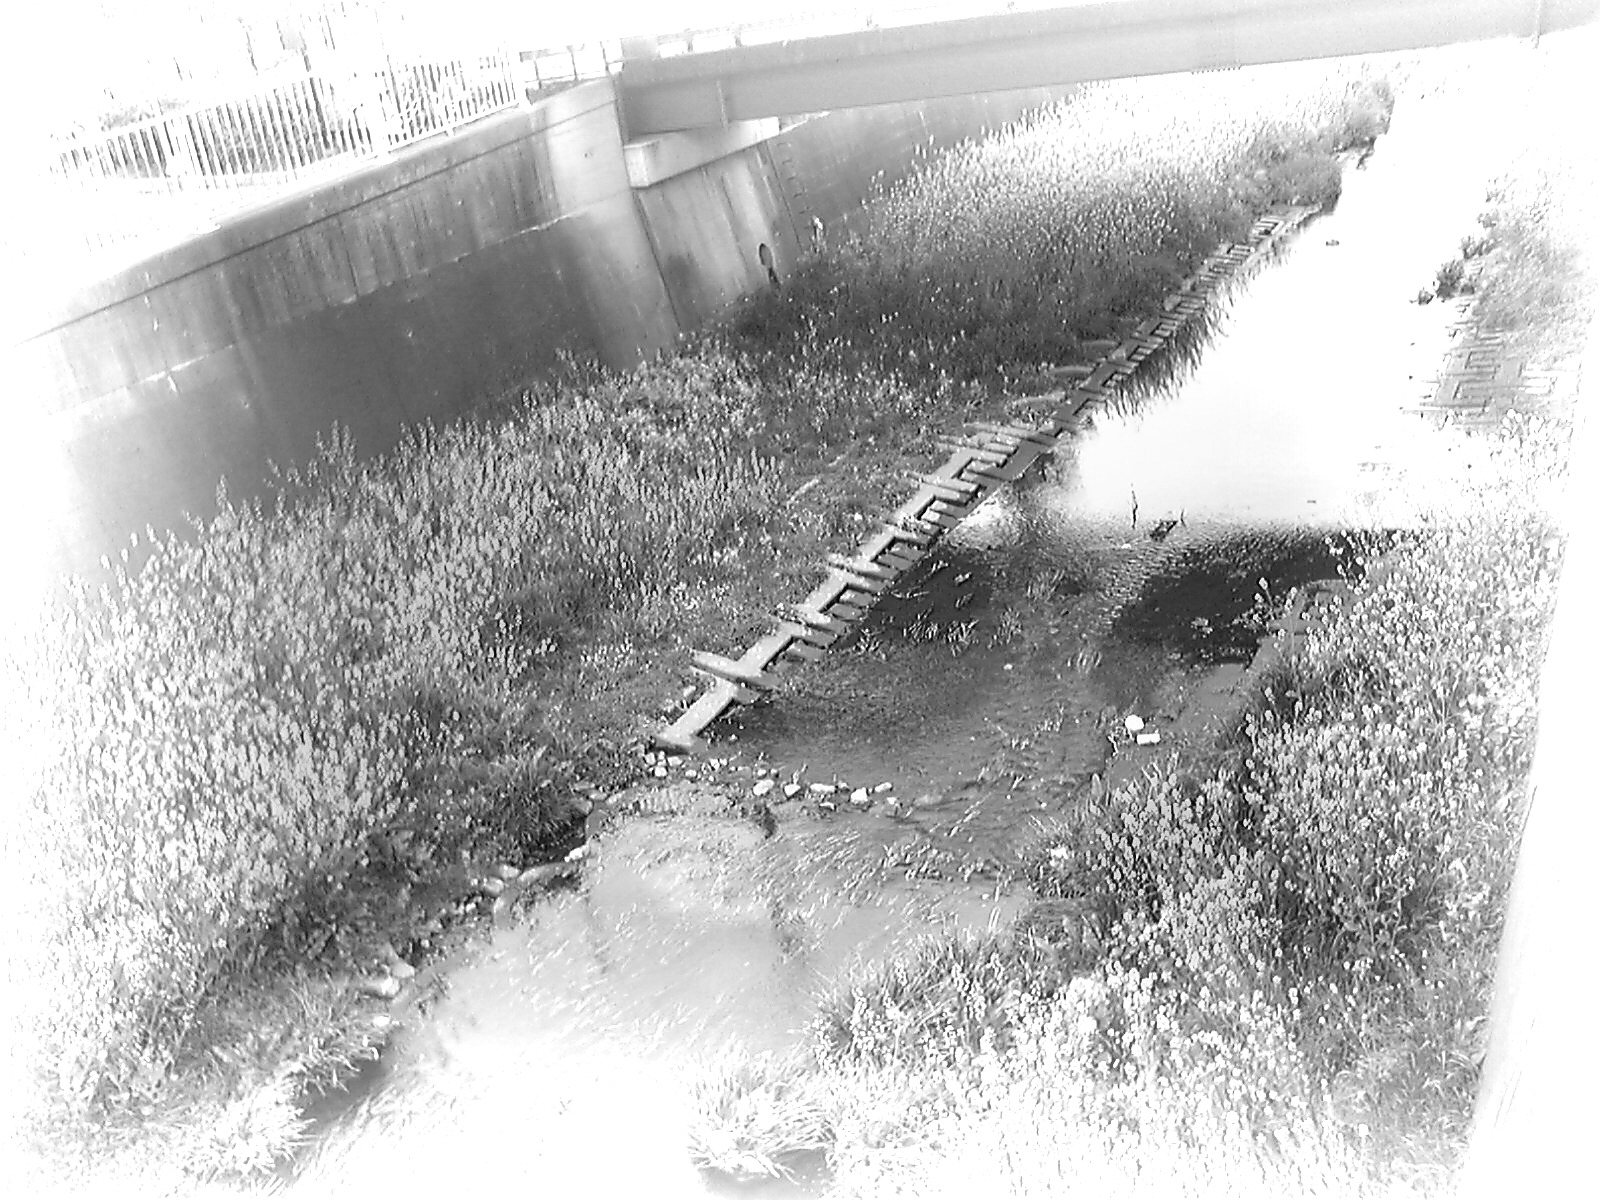
\includegraphics[width=0.58\textwidth,bb=0 0 1600 1200]{img/river.jpg}
\end{wrapfigure}

私が子猫に餌付けする様子を少し遠くから伺う大人たち、
歩行者用のトンネルの裏側の落書き、
川に投げ捨てられて錆びついた自転車、
それくらいのもので、どれも全く毎日見てきたものだ.
トンネルの向こう側に行くと地名が変わり、
多少は街も賑わいも見せてくる.
とは言っても道は細く、
例えばこのスーパーの外は自転車が多く駐輪されて通りにくいことこの上ない.
しかしどうやら今日は休みのようであった.
てっきり年中無休で営業されるものだと思っていたのだけれど.
しかし、店が開いていないのにその前に駐輪されてる自転車の数というのは、
何かを測る指標になるかもしれない、
と思った.

鈍感な私はここでようやく異変に気付いた.
上を見上げると北大阪急行の線路がある.
先程から電車が一本も走っていない気がする.
そういえば開いているお店が一つもないこと、
誰ともすれ違わないこと、
自動車が走っていないこと.
私がこの散歩のささやかなゴールにしている古本屋も当然と言った様子で暗く、
その自動ドアは施錠されて開かなかった.
始めこそ、これはなかなかに珍しい風景に出会ったものだと、呑気に気構え、
私しか居ないこの街を散歩して歩いて回っていた.
だんだんと、不安になり、電車も走っていないのなら、どうやって帰ればいいかと考えた.
いや、そういう問題でもないな.
帰宅するだとかそういう以前の問題かもしれない.
私は薬局前のブロックの上に腰掛けて、
自然と震える足をさすった.

問題が解決するまでには体感でも五分と掛からなかった.
ガラスがぴしゃりと割れる音が聞こえたのだ.
紛れもなく、これは人間の音だと思った.
駆け足になって私は音の発生元を探した.
コンビニのドアが割れていた.
それが誰であったとしても、
私は努めて仲良くなれると思った.\\
「どうやら、こんな真似をしても私のことを捕まえる人はいないと思ったのでね」\\
男は手に持てるだけの袋入りパンを持ち、
まずは盗みをしてることについての弁明をした.
私は努めて愛想よく
「ええ、状況が状況です」
と言って、入り口すぐ近くにあった買い物かごを一つ持って見せた.

何か情報を求めて話をしてみたが、
状況がわからないのは向こうも同じようだった.
男は、アリカワというらしい、
すぐ近所に居を構えているらしく、
家に貯蓄した食べ物が尽きたので外に出たらこんな感じで、それがついさっきだと言う.
初め私は、すぐ近所に家があるからこんなに、この男は落ち着いていられるのだと思ったが、
それもあるが、それよりも、根本的にこの男の性格ゆえらしいと思い始めた.
つまり、こんなことになってラッキーだ、と言わんばかりで.
男は私から受け取ったカゴに手当たりしだいに入れ、ニコリと笑った.
そんなわけで、しばらくはその男の家にお世話になることになったのだ.

ふう、疲れた.

